\section{Code Generation}
\label{sec:implementation_codeGen}
To generate the target code, first, the parse tree is traverse and the source code is translated to an in-memory representation consisting of objects corresponding to different language concept. These concepts can be divided into three different kinds, statements, declarations, and code blocks. All of the objects implement the \texttt{ITranslatable} interface; it requires a translation function that translates the source code representation to the target code representation. In turn, they are often referred to as translatables. The target code representation is a collection of objects that describe an OpenQASM program; they can be translated directly to the textual OpenQASM code. In the following, we discuss the generation of the source code representation from the parse tree, the translation from the source code to the target code representation, and any other utilities that are used in the process.\todo{How are expressions created and evaluated?}

\subsection{Source Code Representation}
\label{sec:implementation_sourceCode}
Similar to the implementation of the semantic analysis, the parse tree is traversed with another custom listener. However, in contrast to the semantic analysis, the code generation listener does not directly interact with a symbol table but uses a separate code generation handler.

The code generation handler facilitates the creation of the source code representation when traversing the parse tree. Firstly, it contains a main code block; this code block is initiated as an empty code block without a parent when the handler is created. Furthermore, it will hold, directly or indirectly, the references to all other source code objects. The second important property is the symbol table. The handler implements different methods for interaction with this table. For example, it contains methods for both pushing and popping scopes as well as guards. Additionally, the handler implants unique functions for each symbol that can be added to the table, with a protected general function. This is done because some symbols need additional logic when they are added to the symbol table. For example, when a register symbol is added to the table, a register declarations is also added to the current code block.

In the code generation listener, similar to the semantic analysis, the scopes and guards are pushed and popped based on the tree traversal. Furthermore, the symbols are also added according to the declarations in the source code. Except for the main code block, all translatables, \ie code blocks, statements and declarations, belong to exactly one code bock. In turn, whenever one is reached in the traversal of the parse tree, the translatable is created and added to the corresponding code block. This code block is always identified as the current code block. Whenever a code block is entered, the current code block is updated to the newly created one. In turn, when a block is exited, the current is set to the parent of the current block.

The first example of a translatable is the register declaration; as described previously, whenever a register symbol is added, the corresponding declaration is added to the current code block. In contrast, statements require more information. For each statement, the relevant symbol information is read from the symbol table based on the given identifier. Furthermore, any additional information is retrieved from the code generation handler. Then, both the symbol and additional information is used to create the statement object. For example, a loop statement requires both the loop iterator symbol and the code block object of its loop body. In turn, since the code block needs to have been traversed, the loop statement is created in the exit function of the loop rule. However, as the code block was already existed, the listener class needs to save the pasted popped scope and retrieve the code block, corresponding to the loop body, from it. The loop iterator can easily be read from the symbol table based on the given identifier. While the type checking ensures the correct type of the symbol in most cases, a code generation exception may be thrown, if the symbol in the table is not a loop iterator. Finally, the loop statement is created and added to the code generation handler and, in turn, to the current code block. The creation of the other statements works similar; however, since the predefined and composite gates are implemented as separate translatable statements, the gate application need to differentiate between the two and create the corresponding statement.

The most basic translatable is the code block. It represents a block of code in the source program and, in turn, contains all statements and declaration contained in the block; they are saved in a list of translatables. Next, the code block object also contains a reference to its parent code block. If the code block is the main block of the program, the parent is set to null. While each variable has a unique identifier, this identifier is only unique in the context of its declaration and an independent context may contain a declaration for the same identifier. Therefore, the identifiers used in the source code may not be usable in the target code. To solve this issue, each declaration is assigned a new unique identifier. The code block contains a dictionary that maps all its declarations to the corresponding unique identifiers. Besides these three properties, the code block implements some functions to add translatables to the list and some utility functions to, \eg, retrieve the unique identifiers for declarations.

Another type of translatables are the declarations. While there are multiple different declarations, \eg register and composite gate declarations, in our source language, most concepts are not translated to a corresponding declaration in the target language; in turn, there currently only exists one possible declaration. However, for extensibility, the compiler contains an abstract declaration class; it include symbol property with a reference to the symbol that is declared by the declaration. The register declaration inherits from the abstract class and is the only required declaration. 

The third group of translatables are statements. Each statement inherits from an abstract statement class. Each statement contains an error context that corresponds to the source code location of the statement. In total, there are six different statements. 

The first two are the different gate application statements, the composite gate statement and the gate application statement. Since the implementation of the translation differs so greatly, they are implemented as two differed statements. Both contain a gate property; however, while the gate property of the composite gate statement is a composite gate, the gate application statements contains a predefined gate in its property. Furthermore, they both contain a parameters property. In this case, while the gate application statement simply saves a list of symbols, the composite gate contains a dictionary that maps the parameter symbols used in the composite gates to the symbols given as arguments.

Next, three statements are related to the control flow of the program. Firstly, the loop statements, contains both the loop iterator symbol and the body of the loop in the form of a code block. Similarly, the quantum if statement also contains a reference to its code block. Additionally, the statement includes a guard property which holds the symbol guarding the execution of the code block. Furthermore, the else statement simply inherits from the if statement and contains no additional properties.

Lastly, in contrast to most other statements, the skip statement does not contain any additional properties. All the different translatables, including the code block, statements, and declarations, are depicted in Fig.~\ref{fig:implementation_uml_translatables}. 

\begin{figure}[htp]
    \centering
    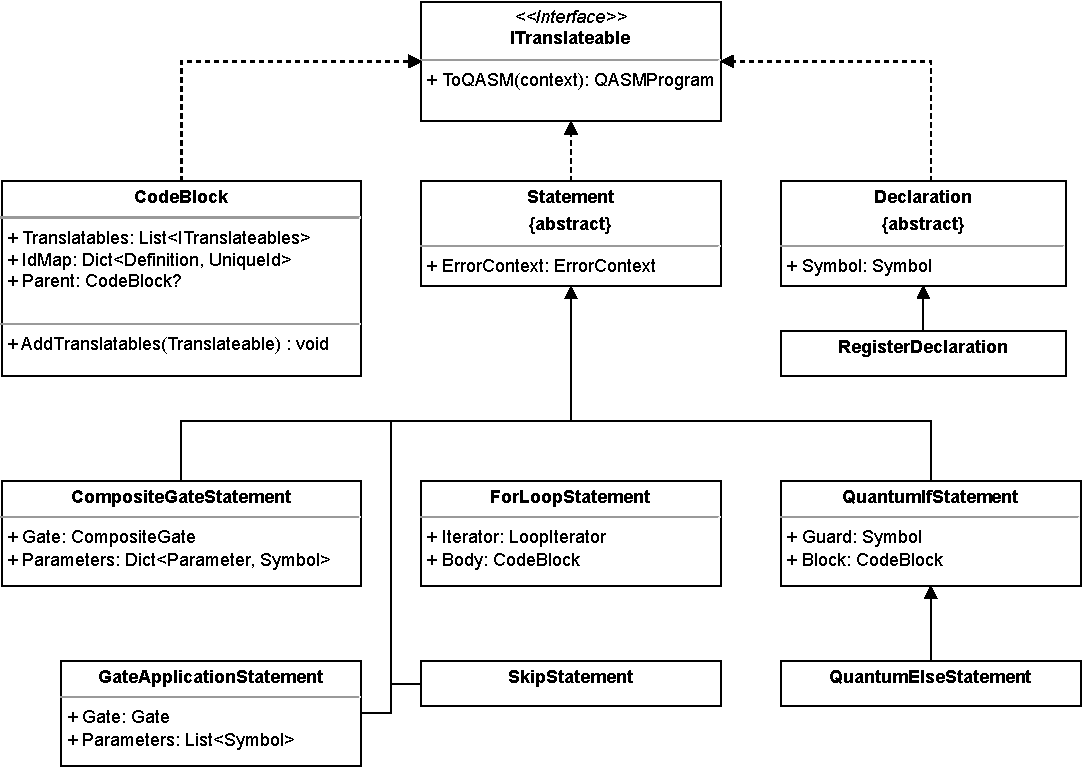
\includegraphics[width=.9\textwidth]{../figures/uml_translateables.pdf}
    \caption{UML diagram of the different translatables.}
    \label{fig:implementation_uml_translatables}
\end{figure}

\subsection{Translation}
\label{sec:implementation_translation}
To create the target code representation, that can be translated to the final program, the translatables, \ie code blocks, declarations, and statements, need to be translated. For this, all translatables implement a translation function, that takes the code generation context and returns the target code representation in the form of a \texttt{QASMProgram} object.

The code generation context contains all additional, relevant information for the code generation that is not already contained in the translatable objects themselves; this may include information that is not known at the time the translatables are created and instead injected when they are translated. The first property is the current block which holds a reference to the code block for which the code is generated. Since all statements must be contained in a block, there must also always exist a current code block. The block, \eg, contains a dictionary that maps the declarations to the corresponding identifiers; this dictionary filled while translating the declarations. Therefore, the information must be injected with the help of the code generation context. 

Similarly, the code generation context holds the symbol table that is generated while creating the source code representation. However, this symbol table may be changed while the code is translated. For example, composite gates are inlined where they are applied. However, the translation of the composite gate require an empty symbol table as they do not have access to any symbols outside the scope of the composite gate. In turn, the translation of the composite gate cannot use the symbol table of its current block, but must create a new one. The symbol table itself is used to retrieve symbol information for, \eg, the evaluation of expressions where it may be used to get the value of a constant symbol.

Lastly, the context contains a dictionary that maps a parameter to a symbol. This is used for the translation of the composite gates. Since there may exist nested composite gates, \ie a composite gate that calls another composite gate, the dictionary contained in each composite gate statement is not sufficient for the translation alone. In turn, for each composite gate translation the corresponding mappings are added to the dictionary.

The translation of any source code representation will always start with a code block translation as it is always the root of a program. However, our target code representation does not contain a code block equivalent. In turn, instead of translating the code block directly, a new program object is created and each translatable, contained in the code block, is translated individually and added to the code block. Then, the resulting program object is returned.

In contrast, the register declaration has an equivalent in the target language. In this case, this is the qubit declaration code. However, as previously described, the identifier that is declared may not be unique. In turn, the symbol table is used to create an identifier that is unique in the resulting program. Futhermore, this identifier is added to the dictionary of the current block so that any reference to the declaration can be mapped to the newly created unique identifier. While the size of a register declaration is given in the form of an expression, the target code objects requires a constant integer value. Therefore, the size expression is also evaluated before the code object is created. 

Of the statements, the skip statement is the easiest to translate; it represents an empty operation and, therefore, is translated by returning an empty program object. Similarly, the gate application statement has a simple translation. Since the target language also contains gate application statements, the translation simply needs to convert the gate and parameters to the target code representation. This can be accomplished with some simple helper functions and look ups. In contrast, the composite gate statement does not have any target code equivalent and is, instead, inlined. In turn, the composite gate translation simply calls the translation for the body code block and injects some parameter mappings. Then, the translation of the body is returned.

The translation of the loop statements is, in principle, similar to the translation of a composite gate; it also contains a code block which is translated. However, the code block is not inlined once but needs to be translated multiple times, each time with a different value for the iterator. To achieve this, both the start index and end index expressions are evaluated. Next, the current value of the iterator is set to the start index and a for loop is executed till the current value is equal to or larger than the end value. For each iteration, the code block is translated and added to a program. At the end, the program consists of the unrolled loop statement and is returned. 

Lastly, the translation of the if and else statements are mostly identical. In our target language, OpenQASM, the desired behavior for both the if and else statement can be accomplished by adding a control and negative control to each gate application statement in the code block respectively. For this, the program object contains a function to add a guard. In this function, all code objects are iterated and the guard is added to each gate application code. For the else statement, a negated guard can easily be added. Therefore, the translation of the if and else statements consists of translating the code block and adding the guard symbol as a possibly negated guard to it. 

\subsection{Target Code Representation}
\label{sec:implementation_targetCode}

\subsection{Expressions}
